
Una buena elección de la tecnología será una condición necesaria, aunque no suficiente, para llevar a cabo un proyecto con éxito.

En esta sección explicaremos los entornos en los que se trabajo a la hora de desarrollar este proyecto, comentando los fundamento usados en ellos. 

\section{Eclipse Java EE IDE for Web Developers Version Neon2 }
Herramienta para desarrolladores  integrado (IDE)  en Java para el desarrollo de software. Fue creado por IBM como sucesor de uno de sus herramientas y ahora esta en manos de la Fundación Eclipse que es quien se encarga de seguir desarrollandolo.
 Esta herramienta de desarrollo es totalmente gratuita por lo que no encarece el precio del proyecto. Se decidió usar esta herramienta por el parecido que tiene con el entorno de Android y sus facilidades para la creación de código.
\begin{figure}
		\centering
		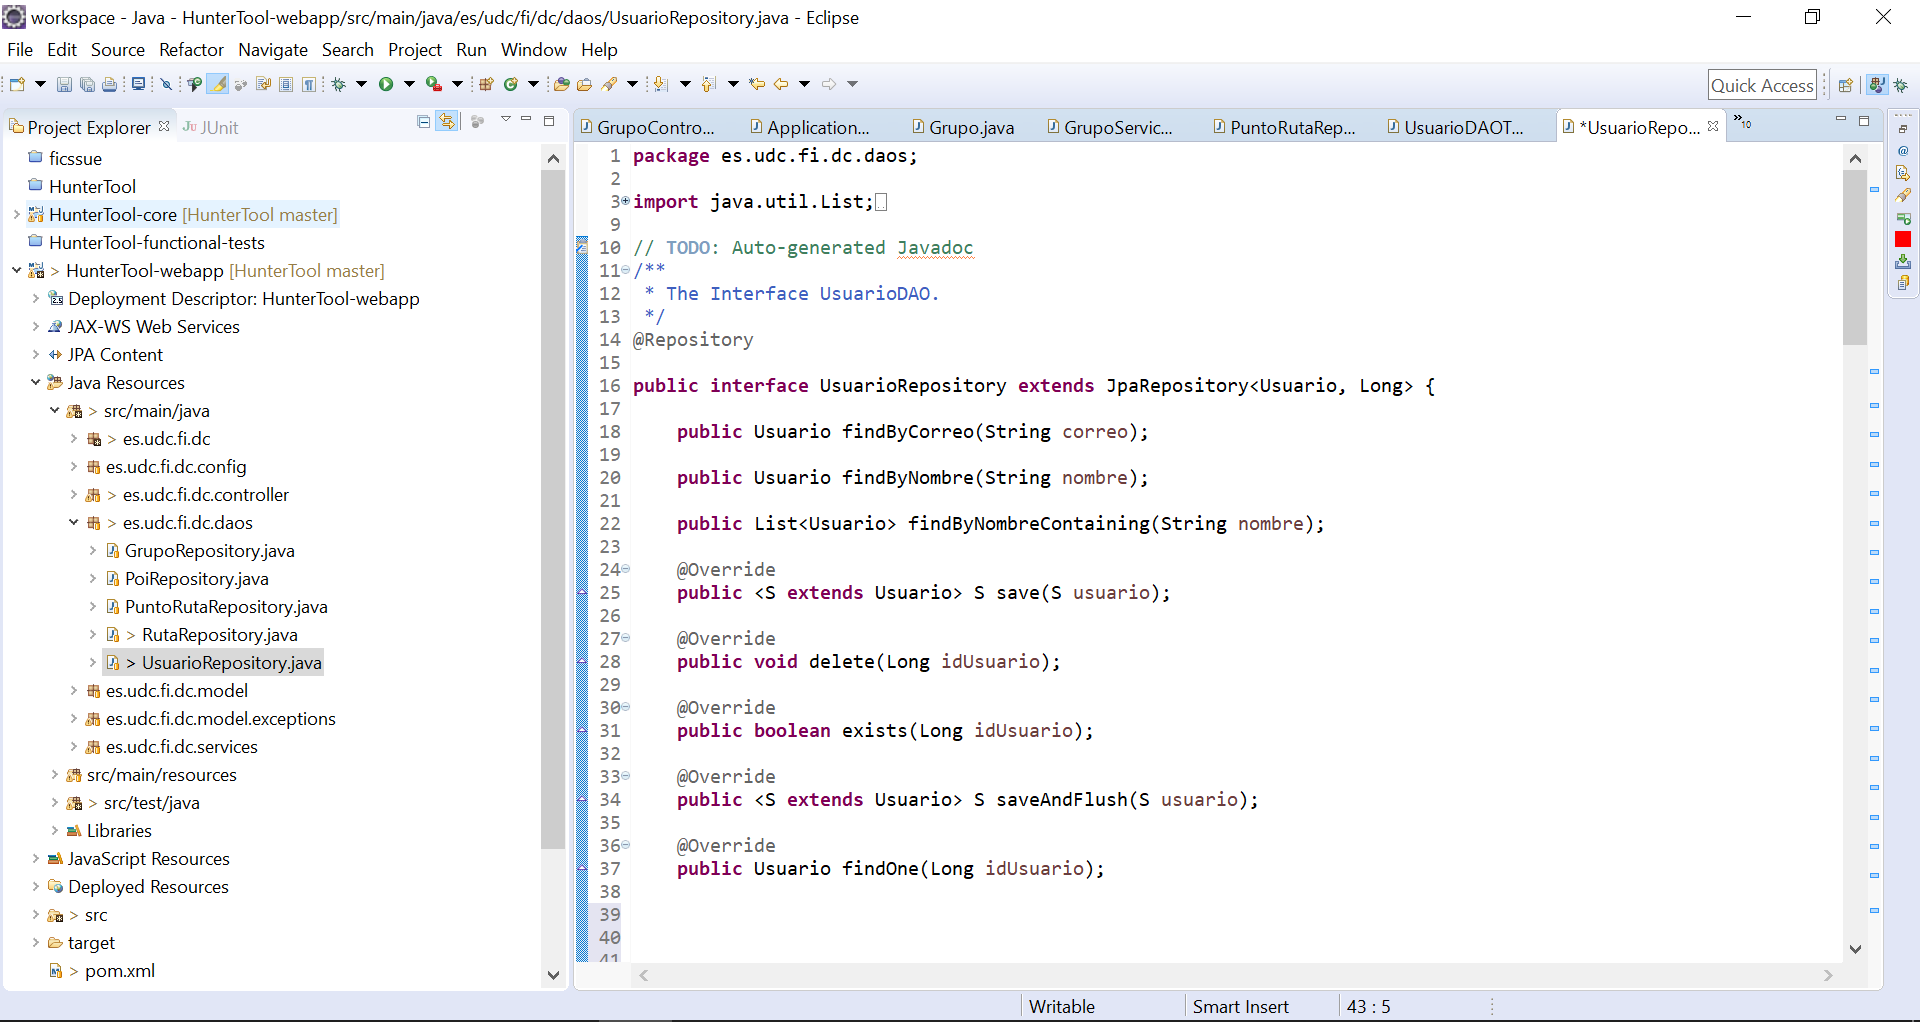
\includegraphics[width=\textwidth] {eclipse.png}
		\caption{Entorno de trabajo Eclipse }
		\label{fig:eclipse}
	\end{figure}
	
	
	
\section{Spring}
Spring es un framework de código abierto que tiene como objetivo ayudar al desarrollador a trabajar con otras APIs de manera más sencilla. Nos proporciona un modelo de programación y configuración integral para aplicaciones empresariales basadas en Java, en cualquier tipo de plataforma de implementación. Simplemente es necesario añadir una dependencia, si se usa Eclipse, en el archivo pom.xml. 

\begin{figure}[H]
		\centering
		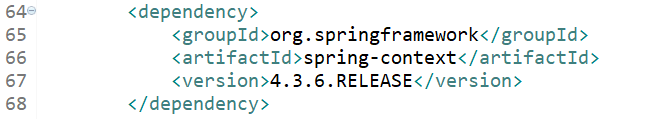
\includegraphics[width=\textwidth] {spring.png}
		\caption{Dependencia de Spring en el pom.xml }\label{fig:spring}
	\end{figure}
	
	
Como funcionalidades principales que nos ofrece y por ello elegí, serían:

\begin{itemize}
\item \textbf{Programación orientada aspectos},paradigma que nos ayuda a eliminar dependencias entre módulos acortando las lineas de código de los servicios para así poder centrarnos en la lógica de la aplicación. Lo que conlleva a reducir  la probabilidad de errores en la codificación o ineficiencias.


\item\textbf{ Inyección de dependencias}, patrón que ayuda a reducir el acoplamiento entre los distintos componentes de la aplicación. Esto lo consigue haciendo que una clase le proporcione a otra sus dependencias haciendo que la otra no tenga que crearlas ella misma. De este modo atreves de un interfaz una clase tienes las dependencias de otra sin tener que preocuparse de la implementacion de las mismas, lo que es favorable para reducir el acoplamiento.

\begin{figure}[H]
		\centering
		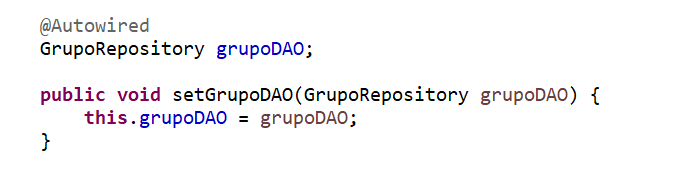
\includegraphics[width=\textwidth] {dao.png}
		\caption{Ejemplo de inyección de dependencia }\label{fig:dao}
	\end{figure}


\end{itemize}


\section{Android Studio}
Android Studio es el entorno de desarrollo integrado (IDE)  oficial para Android que nos ofrece las herramientas más rápidas para crear apps en todas las clases de dispositivos Android.
Ademas se ser una potente herramienta para la creación de código permite:

\begin{itemize}
\item Realizar compilaciones  de nuestro código para comprobar el estado de nuestras variables en los puntos que nosotros le indiquemos sin necesidad de general un APK.
\begin{figure}
		\centering
		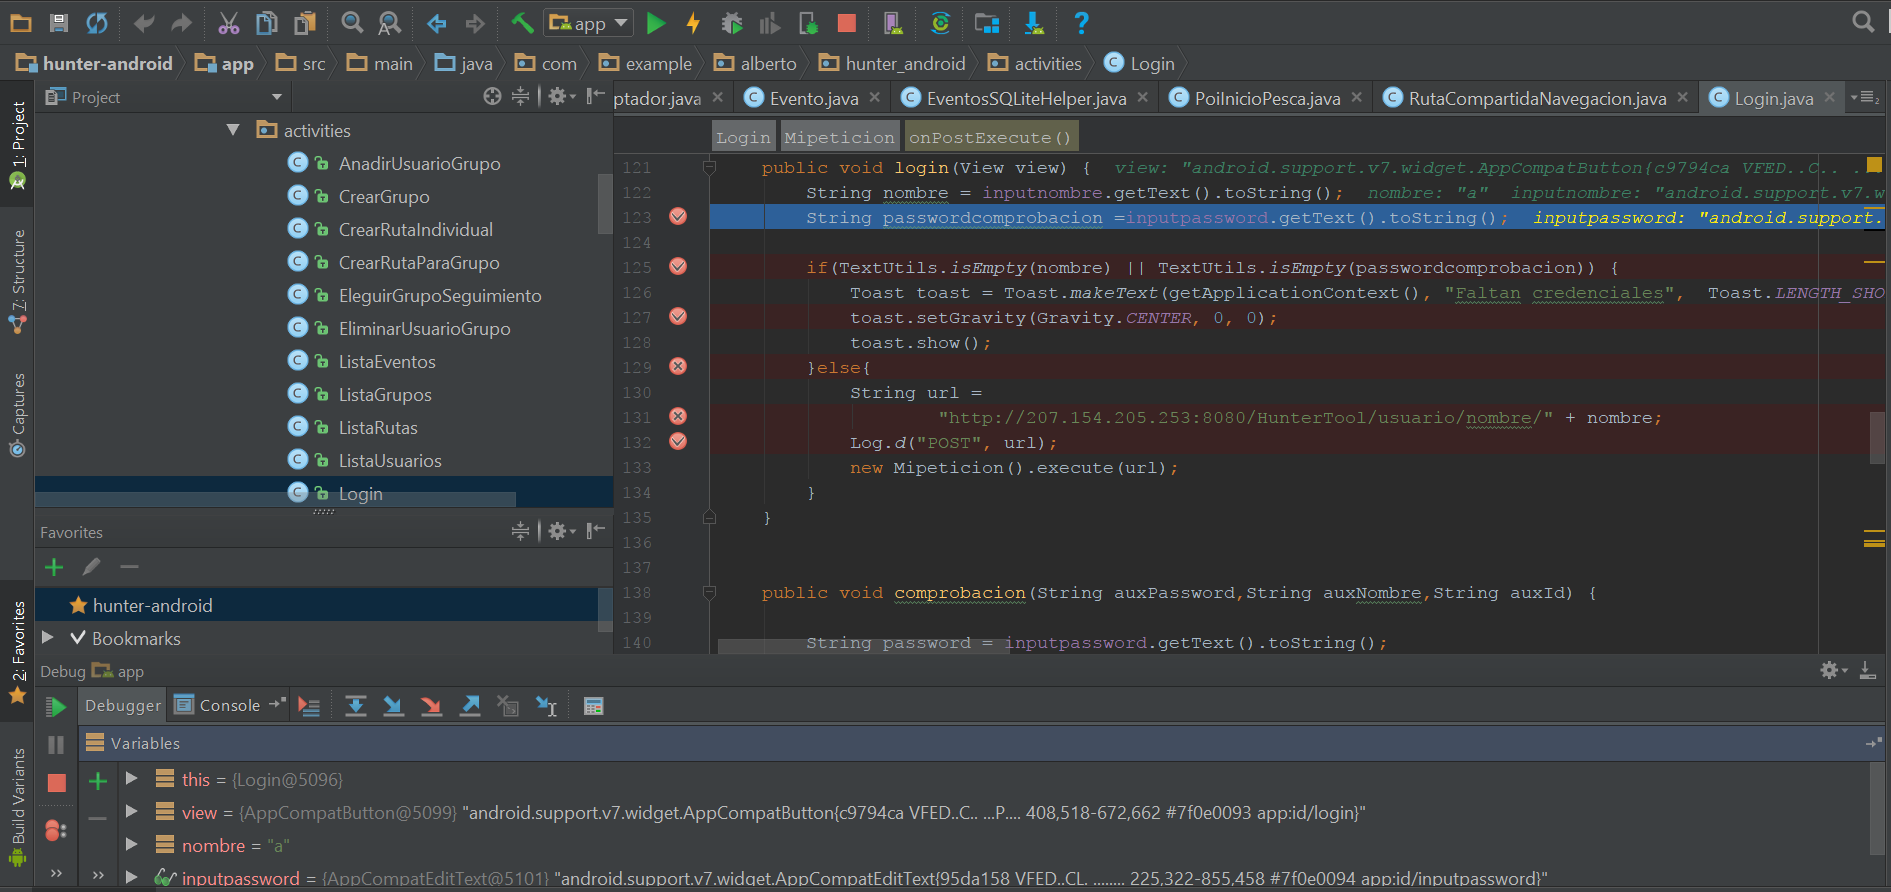
\includegraphics[width=\textwidth] {debug.png}
		\caption{Captura de pantalla realizando app debug }\label{fig:debug}
	\end{figure}

\item Generar un APK (Android Application Package) para la ejecución de nuestra aplicación móvil tanto de forma simulada ayudándonos del simulador que nos proporciona o usando un móvil.
\end{itemize}
\begin{figure}[H]
		\centering
		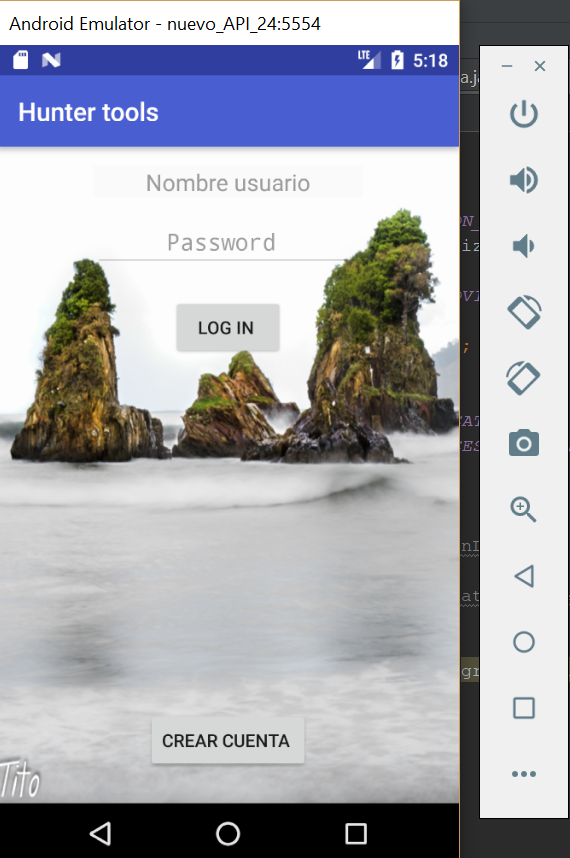
\includegraphics[width=0.6\textwidth] {emulador.png}
		\caption{Emulador de Android con mi aplicación}
		\label{fig:emulador}
	\end{figure}
 
\begin{figure}[H]
		\centering
		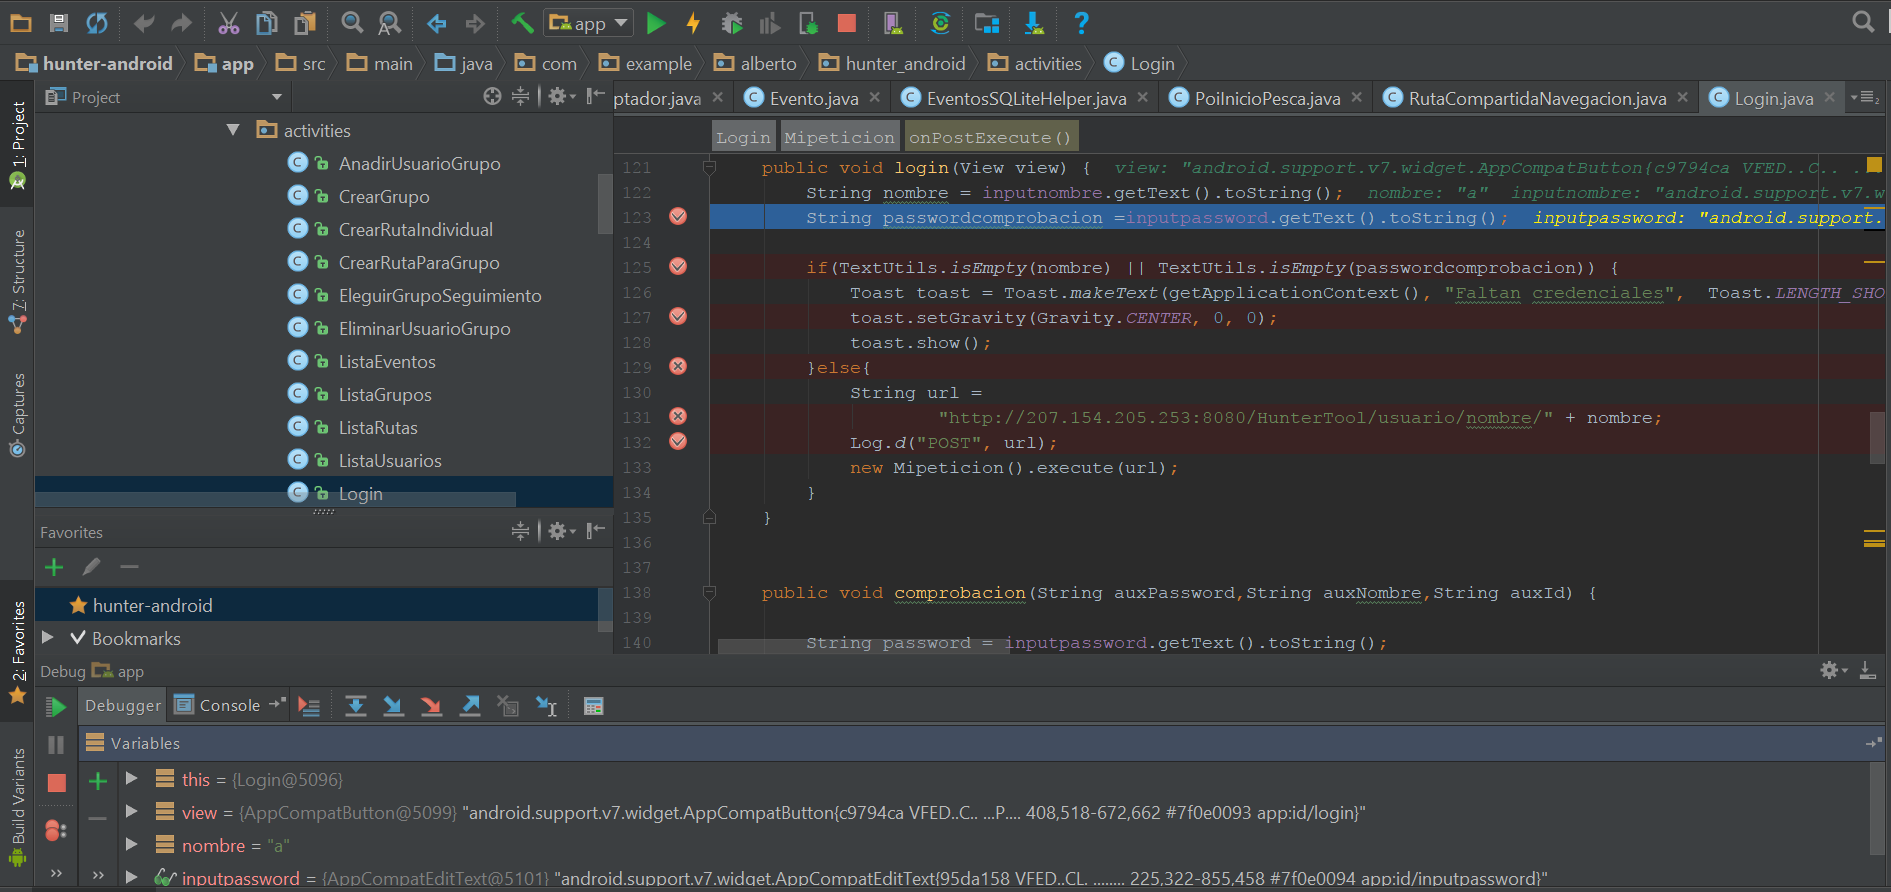
\includegraphics[width=\textwidth] {debug.png}
		\caption{Entorno de trabajo Android Studio }
		\label{fig:debug}
	\end{figure}


\section{Git}
Git es un sofware para ayudarnos con el control de versiones  pensado para el mantenimiento de múltiples versiones de aplicaciones cuando estas tienen un número muy alto de archivos y queremos poder volver a un punto anterior o como copias de seguridad. A su vez Git ofrece 2 opciones para el control de versiones una mediante un interfaz y otra mediante linea de comandos. Se escogió esta opción por las facilidades de uso que ofrece a la hora de realizar lo commits y el fácil nombrado de los mismos cuando queremos actualizar el repositorio.
\section{Maven}
Maven es una herramienta de software para la gestión y construcción de proyectos Java.
 Maven utiliza un Project Object Model (POM) en formato
XML para describir sus dependencias con otros módulos como jpa, firebase o postgrest. Viene con objetivos predefinidos para la compilación del código o su empaquetado. Se escogió por la buena estructuración de los paquetes que genera y por las similitudes que presente frente al Gradle que usaremos en el entorno de desarrollo Android Studio.




\section{Gradle}
Gradle es una herramienta de software para la gestión, construcción de proyectos Android y gestor de dependencias. Ofrece
  herramientas de compilación avanzadas, para automatizar y administrar el proceso de compilación, y al mismo tiempo te permite definir configuraciones de compilación personalizadas.



\section{Jackson}

Jackson es un parseador para el desarrollo de Servicios Web en java. Implementa un conjunto de   herramientas de procesamiento de datos para Java haciendo que el desarrollo de servicios Rest sean más simples. Se eligió esta opción por lo sencillo que hacia el mapeo de objetos en las peticiones a JSON y dado que se usa el framework Spring este parseador ya viene integrado.








\section{JPA/Hibernate}
Hibernate es una herramienta de mapeo objeto-relacional para la plataforma Java que ayuda a la transformación de objetos del modelo a una entidad de la base de datos persistente. Este mapeo ayuda a  no tener que definir la entidad directamente en nuestro gestor de base de datos. Para conseguir esto debemos de usar las anotaciones pertinentes en el entorno de desarrollo (Eclipse) sin necesidad de acceder al gestor de base de datos en ningún momento. Una vez puestas las anotaciones los accesos a datos de la  bases de datos pasan a ser muy sencillos.





\section{PostgreSQL}
PostgreSQL es un gestor de bases de datos objecto-relacional  que permite trabajar con grandes cargas de datos consiguiendo una tolerancia alta a errores.
Se decidió usar este gestor porqué tiene una gran adaptabilidad a otros entornos de trabajo lo que ayuda a ganar agilidad y eficiencia. También nos proporciona  el PgAdmin que facilita la gestión y administración de bases de datos ya sea mediante instrucciones SQL o con ayuda de un entorno gráfico. Permite acceder a todas las funcionalidades de la base de datos, consulta, manipulación y gestión de datos.
\section{JUnit}
JUnit es el framework de testing para Java más extendido.
Permite la ejecución de clases Java para evaluar el comportamiento de los métodos a testar.


\vspace{1cm}

Con estas tecnologías se ha llevado a cabo la construcción de los distintos componentes del sistema siguiendo los pasos que comentaremos en el próximo capítulo.
